\documentclass[12pt]{article}
\usepackage[english]{babel} 
\usepackage{fontspec}
\setmainfont{Free Sans}
\usepackage{fancyhdr}
\usepackage{xcolor}
 
% AMS math et autre
\usepackage{amsmath}
\usepackage{amsfonts}
\usepackage{amssymb}
\usepackage{xspace}
\usepackage{upgreek}
 
\graphicspath{{imgs/}}
\sloppy{}
 
\title{Mathematical model of pual leg epithelium}
 
\author{G. Gay}

\section{Mathematical model of the epithelium}

\subsection{Architecture}

\subsubsection{The elementary cell}

The architecture of the epithelium model consists in a graph containing

\begin{itemize}
\item
  two types of vertices:

  \begin{quote}
  \begin{itemize}
  \itemsep1pt\parskip0pt\parsep0pt
  \item
    The cell centers
  \item
    The appical junctions vertices
  \end{itemize}
  \end{quote}
\item
  and two types of edges:

  \begin{quote}
  \begin{itemize}
  \item
    The junction edges, structuring the apical surface of the epithelium
  \item
    The cell to junction edges linking one cell to its neighbouring
    junction vertices.

    \begin{quote}
    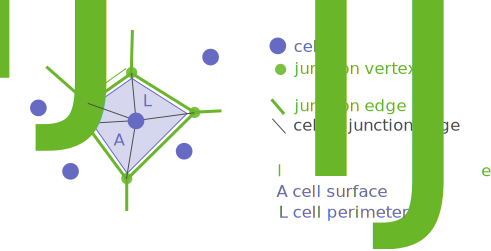
\includegraphics{imgs/one_cell.*}
    \end{quote}
  \end{itemize}
  \end{quote}
\end{itemize}

\subsubsection{Topological modifications}

\begin{itemize}
\itemsep1pt\parskip0pt\parsep0pt
\item
  Cell division
\item
  Type 1 transition
\item
  Cell removal
\end{itemize}

\subsubsection{Locality}

In many aspects of the model, only a local section of the epithelium is
manipulated, most notably during energy minimization.

\subsection{Dynamical aspects}

\subsubsection{3D geometry}

The positions of the vertices are given in two 3D coordinate systems,
Cartesian $(x, y, z)$ and cylindrical $(\rho, \theta, z)$.

Initially, the vertices are distributed over a cylinder centered around
the $z$ axis. The volume of a cell is computed as the sum of the area of
each triangle formed by a junction edge and two cell-to-junction edges
times the height of the cell center. Of course this is an approximation:

$$
\[V_\alpha = \sum_{i,j} A_{\alpha ij} 
   h_\alpha c_{\alpha i} c_{\alpha j} c_{ij}\]
$$

with $c_{uv} = 1$ if vertices $u$ and $v$ are connected and $0$
otherwise, and
$A_{\alpha ij} = \vert \vert \mathbf{r}_{\alpha i} \times \mathbf{ r}_{\alpha j} \vert \vert  / 2$

\subsubsection{Energetical aspects}

The underlying physical properties of the epithelium are an adaptation
of the model proposed by R. Faradhifar et al. {[}Farad{]}\_ generalized
to 3D geometries (constrained for now to deformation of the cylinder)




\paragraph{Total energy of the epithelium}

According to R. Faradhifar et al. in the case of a regular hexagonal
latice, energy is given by:

$$
E = N_{\alpha}\frac{K}{2} (A - A_0)^2 + N\frac{\Gamma}{2} L^2 +
6N\frac{\Lambda}{2}\ell
$$

In our model, the area dependant term is replaced by a volume term. The
cell volume is given by its height $h$ times its area $A$:

$$
E = N_{\alpha}\frac{K_v}{2} (h A - h_0A_0)^2 + N\frac{\Gamma}{2}
L^2 + 6N\frac{\Lambda}{2}\ell
$$

Note that the 3D model is exactly equivalent to the 2D one with a
constant cell height $(h_0 = h = 1)$.

As they did, we define the adimentional contractility
$\bar\Gamma = \Gamma/K_vh_0A_0$ and line tension
$\bar\Lambda = \Lambda /K_v(h_0A_0)^{3/2}$. The normalized energy
$\bar E = E/NK_v(h_0A_0)^2$ then reads:

\bar E = \frac{1}{2} \left(\left(\frac{hA}{h_0A_0}^2 - 1\right)^2 + \frac{\bar\Gamma}{2} \frac{L^2}{h_0A_0} + 6\frac{\bar\Lambda\ell}{\sqrt{h_0A_0}}\right)

The perimeter $L$ of a cell is equal to $6\ell$ and the area $A$ equals
$(3\sqrt{3}/2)\ell^2$. We define a dilatation factor $\delta$ such that
$\delta^2 = hA/(h_0A_0)$. Thus:

$$hA/h_0A_0 = \delta^2 = \frac{3\sqrt{3}}{2} \frac{\ell^2}{h_0A_0}
\Rightarrow  \ell = \sqrt{\frac{2}{3\sqrt{3}}}\delta\sqrt{h_0A_0}$$\]

We define the constant $\mu = 6\left(2/3\sqrt{3}\right)^{1/2}$, then
$\ell = \frac{\mu}{6}\delta\sqrt{h_0A_0}$ and $L^2 =
\mu^2 \delta^2 h_0A_0$

$$\bar E = ((\delta^2 -1)^2 + \bar\Gamma\mu^2\delta^2 + \bar\Lambda\mu\delta) / 2 =  (\delta^4 + (\bar\Gamma\mu^2 - 2)\delta^2 + \bar\Lambda\mu\delta - 1)/2\]

\paragraph{Computation of the gradient}

In order to compute the local minimum of the energy, we calculate its
gradient at junction vertex $i$:
$$
\mathbf{\nabla}_i E = (\frac{\partial E}{\partial x},
                     \frac{\partial E}{\partial y},
                     \frac{\partial E}{\partial z}) \\
= \sum_\alpha \left(K (V_\alpha - V_0) \mathbf{\nabla}_i V_\alpha
 + \Gamma L_\alpha \mathbf{\nabla}_i L_\alpha  \right)c_{i, \alpha} \\
 + \sum_i \Lambda_{ij} \mathbf{\nabla}_i \ell_{ij}
$$




Eaton, S., and Jülicher, F. 2007. \emph{The influence of cell mechanics,
Cell-Cell interactions, and proliferation on epithelial packing.}
Current Biology \textbf{17}:2095-2104.
\url{http://dx.doi.org/10.1016/j.cub.2007.11.049}



%%% Local Variables: 
%%% ispell-local-dictionary: en_US
%%% mode: latex 
%%% TeX-master: t %%%